\documentclass[a4paper,12pt]{article}
\usepackage{graphicx}
\usepackage{float}
\usepackage{listings}
\usepackage{color}
\usepackage{courier}
\usepackage{geometry}
\geometry{margin=1in}
\usepackage{enumitem}
\usepackage{titlesec}

% Define Java syntax highlighting
\definecolor{javared}{rgb}{0.6,0,0}
\definecolor{javagreen}{rgb}{0.25,0.5,0.35}
\definecolor{javapurple}{rgb}{0.5,0,0.35}
\definecolor{javadocblue}{rgb}{0.25,0.35,0.75}
\lstset{
    language=Java,
    basicstyle=\ttfamily\small,
    keywordstyle=\color{javared}\bfseries,
    stringstyle=\color{javagreen},
    commentstyle=\color{javagreen}\itshape,
    morecomment=[s][\color{javadocblue}]{/**}{*/},
    numbers=left,
    numberstyle=\tiny\color{black},
    stepnumber=1,
    numbersep=10pt,
    tabsize=4,
    showspaces=false,
    showstringspaces=false
}

% Custom command for practical title
\newcounter{practicalno} % Create a new counter for practical numbers
\setcounter{practicalno}{-1} % Initialize the counter to 0
\newcommand{\practicaltitle}[1]{
    \stepcounter{practicalno} % Increment the practical number counter
    \newpage
    \begin{center}
        \vspace{1cm}
        \Large\textbf{Practical \thepracticalno} \\
        \vspace{0.5cm}
        \Large\textbf{#1} % Display the title on the next line
        \normalsize\vspace{1cm}
    \end{center}
}

%Redefine \subsection command to use hashtags instead of numbers
\titleformat{\subsection}[block]{\bfseries\large}{\texttt{\#}}{1em}{}
% Redefine \subsubsection command to use arrow instead of numbers
\titleformat{\subsubsection}[block]{\bfseries\normalsize}{\texttt{>}}{1em}{}

\title{\textbf{Java Practical}}
\author{Mayank}
\date{}

% Redefine \subsection command to use hashtags instead of numbers
\titleformat{\subsection}[block]{\bfseries\large}{\texttt{\#}}{1em}{}

\begin{document}

\maketitle

\practicaltitle{Introduction to Java}

\section{Introduction to Java}
JAVA was developed by James Gosling at Sun Microsystems Inc in May 1995 and later acquired by Oracle Corporation. It is a simple programming language. Java makes writing, compiling, and debugging programming easy. It helps to create reusable code and modular programs. Java is a class-based, object-oriented programming language and is designed to have as few implementation dependencies as possible. A general-purpose programming language made for developers to write once run anywhere that is compiled Java code can run on all platforms that support Java. Java applications are compiled to byte code that can run on any Java Virtual Machine. The syntax of Java is similar to C/C++.

Java is widely used for developing applications for desktop, web, and mobile devices. Java is known for its simplicity, robustness, and security features, making it a popular choice for enterprise-level applications.

\section{Java Syntax}
Java syntax is the set of rules defining how a Java program is written and interpreted.
\subsubsection{Code: }
\begin{lstlisting}
public class Syntax {
    public static void main(String[] args) {
        System.out.println("Hello, World!");
    }
}
\end{lstlisting}

\subsection*{public class Main}
\begin{itemize}[leftmargin=2cm]
    \item \textbf{public}: An access modifier indicating that the class is accessible from other classes.
    \item \textbf{class}: A keyword used to define a class in Java.
    \item \textbf{Main}: The name of the class. By convention, class names in Java start with an uppercase letter.
\end{itemize}

\subsection*{public static void main(String[] args)}
\begin{itemize}[leftmargin=2cm]
    \item \textbf{static}: A keyword indicating that the method belongs to the class, not to instances of the class. It can be called without creating an object of the class.
    \item \textbf{void}:  The return type of the method, indicating that it does not return any value.
    \item \textbf{main}: The name of the method. This is the entry point of any Java application.
    \item \textbf{String[] args}: An array of String arguments passed to the method. These are command-line arguments.
\end{itemize}

\subsection*{System.out.println("Hello, World!")}
\begin{itemize}[leftmargin=2cm]
    \item \textbf{System}: A built-in class in the \texttt{java.lang} package.
    \item \textbf{out}: A static field in the \textbf{System} class, which is an instance of \textbf{PrintStream}.
    \item \textbf{println}: A method of \textbf{PrintStream} that prints a message to the standard output (usually the console) followed by a newline.
    \item \textbf{"Hello, World!"}: A string literal that is the message to be printed.
\end{itemize}


\section{Variables in Java}
Variables are containers for storing data values. In Java, every variable must be declared before it is used. A variable declaration includes the data type followed by the variable name. Java supports different types of variables, including:
\begin{itemize}[leftmargin=2cm]
    \item \textbf{Local Variables}: Declared inside a method and accessible only within that method.
    \item \textbf{Instance Variables}: Declared inside a class but outside any method. They are accessible from any method in the class.
    \item \textbf{Static Variables}: Declared with the \texttt{static} keyword. These are shared among all instances of the class.
\end{itemize}


\setcounter{section}{0}
\practicaltitle{Handling Various Data Types}

\section{Data Types in Java}
Java has two categories of data types: \textbf{Primitive Data Types} and \textbf{Reference/Object Data Types}.

\subsection{Primitive Data Types}
Primitive data types are the most basic data types available in Java.
\subsubsection{Code: }
\begin{lstlisting}
public class Data {
    public static void main(String[] args) {
        int myNum = 5;               
        float myFloatNum = 5.99f;
        double myDoubNum = 5.9999d;  
        char myLetter = 'D';        
        boolean myBool = true;       
        String myText = "Hello";     

        System.out.println(myNum);
        System.out.println(myFloatNum);
        System.out.println(myDoubNum);
        System.out.println(myLetter);
        System.out.println(myBool);
        System.out.println(myText);
    }
}
\end{lstlisting}

\begin{figure}[H]
    \centering
    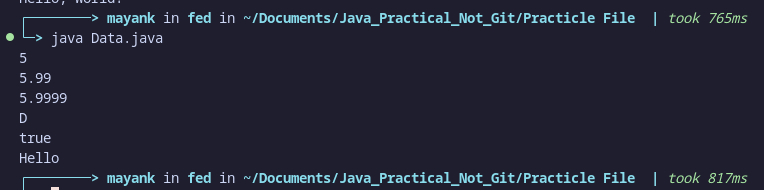
\includegraphics[width=0.9\linewidth]{images/DataOutput.png}
    \caption{Primitve Data Types}
    \label{fig:sample_image}
\end{figure}

\begin{itemize}[leftmargin=2cm]
    \item \textbf{byte}: 8-bit signed integer. Range: -128 to 127.
    \item \textbf{short}: 16-bit signed integer. Range: -32,768 to 32,767.
    \item \textbf{int}: 32-bit signed integer. Range: -2\textsuperscript{31} to 2\textsuperscript{31}-1.
    \item \textbf{long}: 64-bit signed integer. Range: -2\textsuperscript{63} to 2\textsuperscript{63}-1.
    \item \textbf{float}: 32-bit floating-point number.
    \item \textbf{double}: 64-bit floating-point number.
    \item \textbf{char}: 16-bit Unicode character.
    \item \textbf{boolean}: Represents two values: true and false.
\end{itemize}

\subsection{Non Primitive Data Types}
Reference types in Java are Strings and arrays:
\subsubsection{Code: }
\begin{lstlisting}
public class NonPrimitive {
    public static void main(String[] args) {
        // String Data Type
        String stringVar = "Hello, Java!";
        System.out.println("\nString Data Type:");
        System.out.println("String: " + stringVar);

        // Array Data Type
        int[] intArray = {1, 2, 3, 4, 5};
        System.out.println("\nArray Data Type:");
        System.out.print("intArray: ");
        for (int num : intArray) {
            System.out.print(num + " ");
        }
        System.out.println();
    }
}  
\end{lstlisting}

\begin{figure}[H]
    \centering
    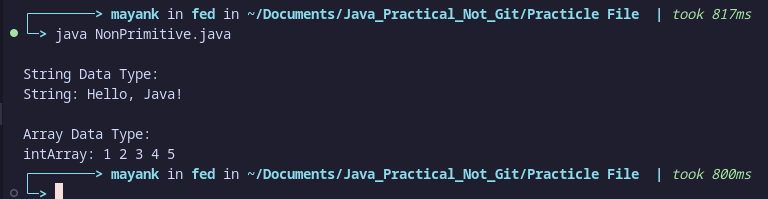
\includegraphics[width=0.9\linewidth]{images/NonPrimData.png}
    \caption{Non-Primitve Data Types}
    \label{fig:sample_image}
\end{figure}

\begin{itemize}[leftmargin=2cm]
    \item \textbf{Strings}: Sequences of characters.
    \item \textbf{Arrays}: Containers that hold multiple values of the same type.
\end{itemize}

\setcounter{section}{0}

\practicaltitle{Type casting}
Type casting is when you assign a value of one primitive data type to another type. There are two types of type casting, implicit typecasting and explicit typecasting which are explained below:

\section{Implicit Type Casting}
Implicit type casting is done automatically when passing a smaller size type to a larger size type.
\begin{center}
    \fbox{
        \parbox{0.9\linewidth}{
            \centering
            \texttt{byte $\rightarrow$ short $\rightarrow$ char $\rightarrow$ int $\rightarrow$ long $\rightarrow$ float $\rightarrow$ double}
        }
    }
\end{center}
\subsubsection{Code: }
\begin{lstlisting}
public class Implicit {
    public static void main(String[] args) {
        int myInt = 9;
        double myDouble = myInt; // Automatic casting: int to double
        System.out.println(myInt); // Outputs 9
        System.out.println(myDouble); // Outputs 9.0
    }
}    
\end{lstlisting}
\subsubsection{Output: }
\begin{figure}[H]
    \centering
    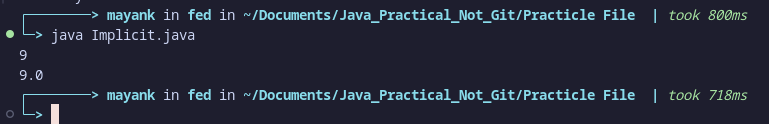
\includegraphics[width=0.9\linewidth]{images/ImplicitOut.png}
    \caption{Implicit Type Conversion}
    \label{fig:sample_image}
\end{figure}

\section{Explicit Type Casting}
Explicit type casting must be done manually by placing the type in parentheses () in front of the value.
\begin{center}
    \fbox{
        \parbox{0.9\linewidth}{
            \centering
            \texttt{double $\rightarrow$ float $\rightarrow$ long $\rightarrow$ int $\rightarrow$ char $\rightarrow$ short $\rightarrow$ byte}
        }
    }
\end{center}
\begin{lstlisting}
public class Explicit {
    public static void main(String[] args) {
        double myDouble = 9.78d;
        int myInt = (int) myDouble; // Manual casting: double to int
    
        System.out.println(myDouble);   // Outputs 9.78
        System.out.println(myInt);      // Outputs 9
    }
}
\end{lstlisting}
\subsubsection{Output: }
\begin{figure}[H]
    \centering
    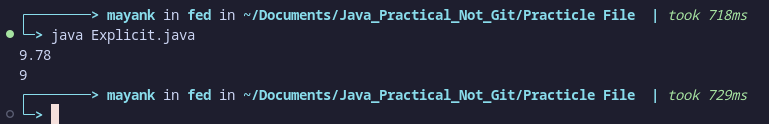
\includegraphics[width=0.9\linewidth]{images/ExplicitOut.png}
    \caption{Explicit Type Conversion}
    \label{fig:sample_image}
\end{figure}

\setcounter{section}{0}

\practicaltitle{Array 1D and 2D}

\section{1-Dimensional Array}
Arrays are used to store multiple values in a single variable, instead of declaring separate variables for each value.
\subsubsection{Code: }
\begin{lstlisting}
public class Array {
    public static void main(String[] args) {
        String[] cars = {"Volvo", "BMW", "Ford", "Mazda"};
        System.out.println(cars[0]); 
        System.out.println(cars[1]); 
        System.out.println(cars[2]); 
        System.out.println(cars[3]); 
        // Changing an element of an array
        cars[0] = "audi";
        System.out.println(cars[0]); 
        // Length of an array
        System.out.println(cars.length);
        // Loop through an array
        for (String arr  : cars) {
            System.out.println(arr);
        }
    }
}  
\end{lstlisting}
\subsubsection{Output: }
\begin{figure}[H]
    \centering
    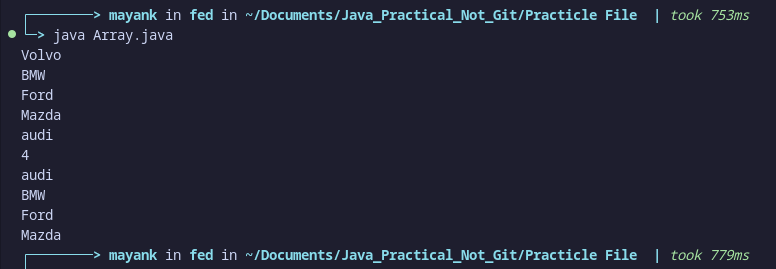
\includegraphics[width=0.9\linewidth]{images/output2.png}
    \caption{output of 1-D array}
    \label{fig:sample_image}
\end{figure}

\section{Multi Dimensional Array}
A multidimensional array is an array of arrays. Multidimensional arrays are useful when you want to store data as a tabular form, like a table with rows and columns.
\subsubsection{Code: }
\begin{lstlisting}
    // Program for Multi-Dimensional Array

public class Array2D {
    public static void main(String[] args) {
        int[][] my2DArr = {{10, 20, 30, 40}, {50, 60, 70}};
        // Accessing Elemensts of array
        System.out.println(my2DArr[0][0]); // 10
        System.out.println(my2DArr[1][2]); // 70
        // change element of array
        my2DArr[0][0] = 100;
        System.out.println(my2DArr[0][0]); //100

        // Loop through a multi dimensional array
        System.out.println("Looping through an array");
        for (int[] row : my2DArr) {
            for(int i : row) {
                System.out.println(i);
            }
        }
    }
}
  
\end{lstlisting}
\subsubsection{Output: }
\begin{figure}[H]
    \centering
    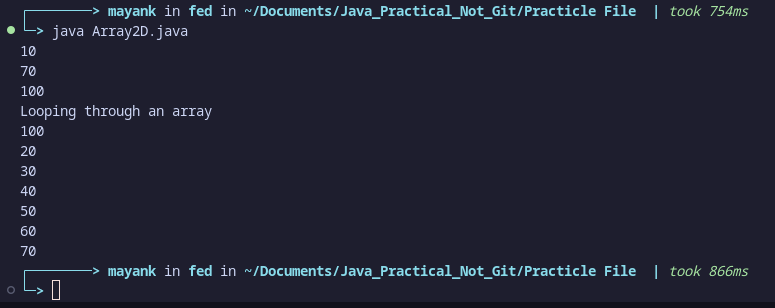
\includegraphics[width=0.9\linewidth]{images/output3.png}
    \caption{output of Multi-D array}
    \label{fig:sample_image}
\end{figure}

\setcounter{section}{0}

\practicaltitle{Various Control Strucutures}

\section{For loop}
For loop provides a concise way of writing the loop structure. Unlike a while loop, a
for statement consumes the initialization, condition and increment/decrement in one line
thereby providing a shorter, easy to debug structure of looping.
\subsubsection{Code: }
\begin{lstlisting}
import java.util.Scanner;

public class ForLoop {
    public static void main(String[] args) {
        Scanner sc = new Scanner(System.in);
        System.out.print("Enter a number: ");
        int n = sc.nextInt();
        for (int i = 0; i < n; i++) {
            System.out.print(i + " ");
        }
        System.out.println();
    }
}
\end{lstlisting}
\subsubsection{Output: }
\begin{figure}[H]
    \centering
    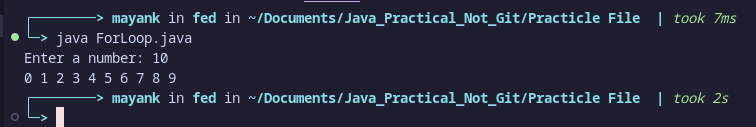
\includegraphics[width=0.9\linewidth]{images/ForOut.png}
    \caption{output of for loop}
    \label{fig:sample_image}
\end{figure}

\section{While loop}
A while loop is a control flow statement that allows code to be executed repeatedly
based on a given Boolean condition. The while loop can be thought of as a repeating if
statement.
\subsubsection{Code: }
\begin{lstlisting}
import java.util.Scanner;

public class WhileLoop {

    public static void main(String[] args) {
// Sum of first n numbers
        Scanner sc = new Scanner(System.in);
        System.out.print("Enter a number: ");
        int n = sc.nextInt();
        int sum = 0;
        while (n > 0) {
            sum += n--;
        }
        System.out.println(sum);
    }
}
\end{lstlisting}
\subsubsection{Output: }
\begin{figure}[H]
    \centering
    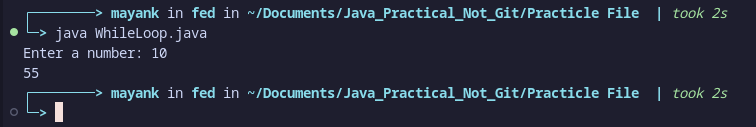
\includegraphics[width=0.9\linewidth]{images/WhileOut.png}
    \caption{output of while loop}
    \label{fig:sample_image}
\end{figure}

\section{Do-While loop}
Do-While loop is similar to while loop with only difference that it checks for condition
after executing the statements, and therefore is an example of Exit Control Loop.
\subsubsection{Code: }
\begin{lstlisting}
import java.util.Scanner;

public class DoWhile {
    public static void main(String[] args) {
        // Sum of first n numbers
        Scanner sc = new Scanner(System.in);
        System.out.print("Enter a number: ");
        int n = sc.nextInt();
        int sum = 0;
        do {
            sum += n--;
        } while (n > 0);
        System.out.println(sum);
    }
}
\end{lstlisting}
\subsubsection{Output: }
\begin{figure}[H]
    \centering
    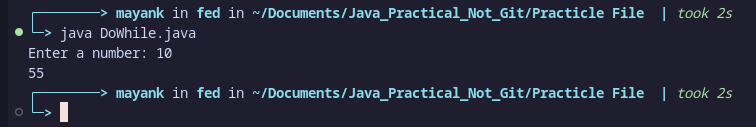
\includegraphics[width=0.9\linewidth]{images/image.png}
    \caption{output of do-while loop}
    \label{fig:sample_image}
\end{figure}

\setcounter{section}{0}

\practicaltitle{Various Decision Strucutures}

\section{The IF statement}
Use the if statement to specify a block of Java code to be executed if a condition is true.
\subsubsection{Code: }
\begin{lstlisting}
public class If {
    public static void main(String[] args) {
        if (20 > 18) {
            System.out.println("20 is greater than 18");
        }
    }
}    
\end{lstlisting}
\subsubsection{Output: }
\begin{figure}[H]
    \centering
    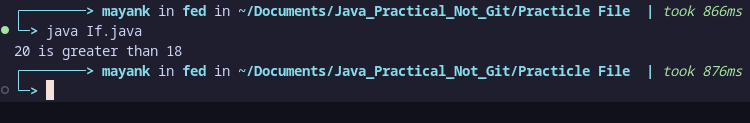
\includegraphics[width=0.9\linewidth]{images/output4.png}
    \caption{output of if statement}
    \label{fig:sample_image}
\end{figure}

\section{The IF-Else statement}
Executes one block of code if its condition evaluates to true, and another block of code if it evaluates to false.
\subsubsection{Code: }
\begin{lstlisting}
public class IfElse {
    public static void main(String[] args) {
        int time = 20;
        if (time < 18) {
            System.out.println("Good day.");
        } else {
            System.out.println("Good evening.");
        }
    }
}    
\end{lstlisting}
\subsubsection{Output: }
\begin{figure}[H]
    \centering
    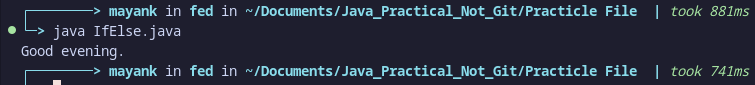
\includegraphics[width=0.9\linewidth]{images/output5.png}
    \caption{output of if-else statement}
    \label{fig:sample_image}
\end{figure}

\section{The IF-Else ladder}
Executes one block of code if its condition evaluates to true, and then checks other
coditions given in else if statements if it is false, or executes the last else block if nothing
is true
\subsubsection{Code: }
\begin{lstlisting}
import java.util.Scanner;

public class IfElseLad {
    public static void main(String[] args) {
        Scanner sc = new Scanner(System.in);
        System.out.print("Enter age -> ");
        int age = sc.nextInt();
        if (age < 12) {
            System.out.println("Child"); 
        }else if (age < 18) {
            System.out.println("Teenager"); 
        }else {
            System.out.println("Adult");
        }
    }
}
\end{lstlisting}
\subsubsection{Output: }
\begin{figure}[H]
    \centering
    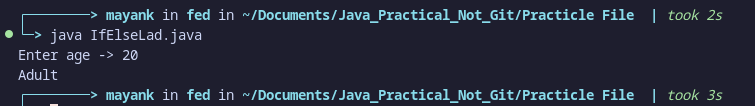
\includegraphics[width=0.9\linewidth]{images/IfElseLad.png}
    \caption{output of if-else-ladder statement}
    \label{fig:sample_image}
\end{figure}

\section{Nested If-Else}
We can put If-Else statements inside otehr If-Else statemetns in order to build more
complex logic
\subsubsection{Code: }
\begin{lstlisting}
import java.util.Scanner;

public class NestedIf {
    public static void main(String[] args) {
        Scanner sc = new Scanner(System.in);
        System.out.print("Enter a -> ");
        int a = sc.nextInt();
        System.out.print("Enter b -> ");
        int b = sc.nextInt();
        System.out.print("Enter c -> ");
        int c = sc.nextInt();
        if (a > b) {
            if (a > c) {
                System.out.println("A is greatest"); 
            }else {
                System.out.println("C is greatest");
            }
        } else {
            if (b > c) {
                System.out.println("B is greatest"); 
            }else {
                System.out.println("C is greatest");
            }
        }
    }
}    
\end{lstlisting}
\subsubsection{Output: }
\begin{figure}[H]
    \centering
    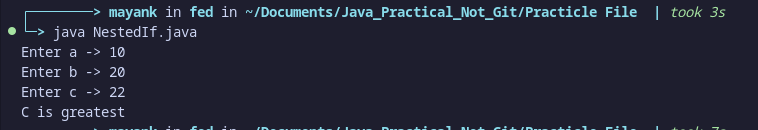
\includegraphics[width=0.9\linewidth]{images/NestOut.png}
    \caption{output of nested-if statement}
    \label{fig:sample_image}
\end{figure}

\section{Switch statement}
The switch statement in Java is a multi-way branch statement. In simple words, the Java
switch statement executes one statement from multiple conditions.
\subsubsection{Code: }
\begin{lstlisting}
import java.util.Scanner;

public class Switch {
    public static void main(String[] args) {
        Scanner sc = new Scanner(System.in);
        System.out.print("Enter a number: ");
        int day = sc.nextInt();
        switch (day) {
            case 1:
                System.out.println("Sunday");
                break;
            case 2:
                System.out.println("Monday");
                break;
            case 3:
                System.out.println("Tuesday");
                break;
            case 4:
                System.out.println("Wednesday");
                break;
            case 5:
                System.out.println("Thursday");
                break;
            case 6:
                System.out.println("Friday");
                break;
            case 7:
                System.out.println("Saturday");
                break;
            default:
                System.out.println("Invalid day");
        }
    }
}
\end{lstlisting}
\subsubsection{Output: }
\begin{figure}[H]
    \centering
    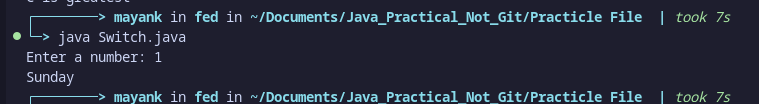
\includegraphics[width=0.9\linewidth]{images/SwitchOut.png}
    \caption{output of switch statement}
    \label{fig:sample_image}
\end{figure}

\setcounter{section}{0}

\practicaltitle{Recursion}
Recursion is the technique of making a function call itself. This technique provides a way to break complicated problems down into simple problems which are easier to solve.

\section{Example of Recursion}
\subsection{Code: }
\begin{lstlisting}
public class Recursion {
    public static void main(String[] args) {
        int result = sum(10);
        System.out.println(result);
    }
    public static int sum(int k) {
        if (k > 0) {
        return k + sum(k - 1);
        } else {
        return 0;
        }
    }
}
\end{lstlisting}
\subsubsection{Output: }
\begin{figure}[H]
    \centering
    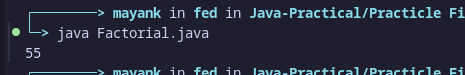
\includegraphics[width=0.9\linewidth]{images/RecExp.png}
    \caption{Recursion Example}
    \label{fig:sample_image}
\end{figure}

\section{Factorial of a number using Recursion}
\subsection{Code: }
\begin{lstlisting}
public class Factorial {
    static int factorial(int n) {
        if (n == 0 || n == 1)
            return 1;
        return n * factorial(n - 1);
    }
    public static void main(String[] args) {
        int ans = factorial(5);
        System.out.println("Factorial of 5 is :" + ans);
    }
}   
\end{lstlisting}
\subsubsection{Output: }
\begin{figure}[H]
    \centering
    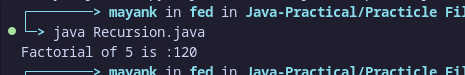
\includegraphics[width=0.9\linewidth]{images/RecursionOut.png}
    \caption{Factorial using example}
    \label{fig:sample_image}
\end{figure}

\setcounter{section}{0}

% \practicaltitle{Practical 2: Type casting}
\practicaltitle{Method Overloading by passing objects as arguments}
In object-oriented programming, method overloading is a feature that allows you to define multiple methods with the same name but different parameters. In the context of passing objects as arguments, method overloading can be used to handle different types or classes of objects.

\section{Example of Method Overloading by passing objects as arguments}
\subsection{Code: }
\begin{lstlisting}
class Circle {
    double radius;
    Circle(double radius) {
        this.radius = radius;
    }
}

class Rectangle {
    double length, width;
    Rectangle(double length, double width) {
        this.length = length;
        this.width = width;
    }
}

class AreaCalculator {
    double calculateArea(Circle circle) {
        return Math.PI * circle.radius * circle.radius;
    }
    double calculateArea(Rectangle rectangle) {
        return rectangle.length * rectangle.width;
    }
}

public class MOPOAA {
    public static void main(String[] args) {
        Circle circle = new Circle(5);
        Rectangle rectangle = new Rectangle(4, 6);
        AreaCalculator calculator = new AreaCalculator();
        System.out.println
        ("Area of Circle: "+calculator.calculateArea(circle));
        System.out.println
        ("Area of Rectangle:"+calculator.calculateArea(rectangle));
    }
}    
\end{lstlisting}
\subsubsection{Output: }
\begin{figure}[H]
    \centering
    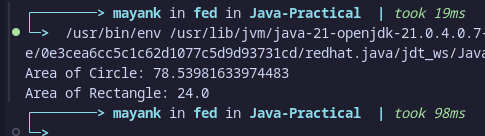
\includegraphics[width=0.9\linewidth]{images/MOPOAA.png}
    \caption{Method Overloading by passing objects as arguments}
    \label{fig:sample_image}
\end{figure}

\setcounter{section}{0}

\practicaltitle{Constructor Overloading by passing objects as arguments}
Constructor overloading in object-oriented programming allows a class to have multiple constructors with different parameter lists. This enables the creation of objects in different ways. When you overload constructors by passing objects as arguments, you can create new objects based on existing objects.

\section{Example of Constructor Overloading by passing objects as arguments}
\subsection{Code: }
\begin{lstlisting}
class Book {
    String title;
    String author;
    int pages;
    // Constructor 1: No arguments
    Book() {
        this.title = "Unknown";
        this.author = "Unknown";
        this.pages = 0;
    }
    // Constructor 2: Passing title, author, and pages
    Book(String title, String author, int pages) {
        this.title = title;
        this.author = author;
        this.pages = pages;
    }
    /*
    Constructor 3: Passing an existing Book object
    (copy constructor)
    */
    Book(Book existingBook) {
        this.title = existingBook.title;
        this.author = existingBook.author;
        this.pages = existingBook.pages;
    }
    void displayDetails() {
        System.out.println("Title: " + title);
        System.out.println("Author: " + author);
        System.out.println("Pages: " + pages);
    }
}

public class COBPOAA {
    public static void main(String[] args) {
        // Using Constructor 1
        Book book1 = new Book();
        System.out.println("Book 1 details:");
        book1.displayDetails();

        // Using Constructor 2
        Book book2 = new Book("1984", "George Orwell", 328);
        System.out.println("\nBook 2 details:");
        book2.displayDetails();

        // Using Constructor 3 (Copy Constructor)
        Book book3 = new Book(book2);
        System.out.println
        ("\nBook 3 details (copied from Book 2):");
        book3.displayDetails();
    }
}    
\end{lstlisting}
\subsubsection{Output: }
\begin{figure}[H]
    \centering
    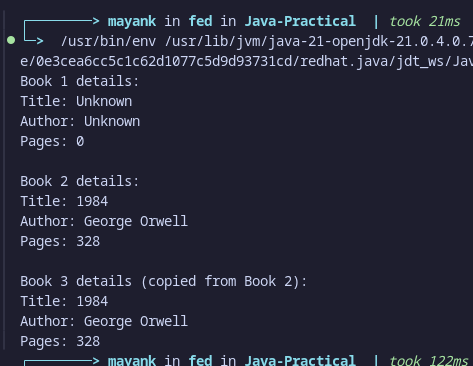
\includegraphics[width=0.9\linewidth]{images/COBPAA.png}
    \caption{Constructor Overloading by passing objects as arguments}
    \label{fig:sample_image}
\end{figure}

\setcounter{section}{0}
\practicaltitle{Access Control and the Usage of Static, Final, and Finalize}

In Java, access control mechanisms and the usage of keywords such as \texttt{static}, \texttt{final}, and the method \texttt{finalize()} are essential components of object-oriented programming. They help in controlling the visibility of class members, managing shared resources, and enhancing performance.

\section{Access Control}
Java provides four types of access control modifiers:
\begin{itemize}
  \item \textbf{Public:} Members are accessible from any other class.
  \item \textbf{Protected:} Members are accessible within the same package and by subclasses.
  \item \textbf{Default:} (No modifier) Members are accessible within the same package.
  \item \textbf{Private:} Members are accessible only within the class itself.
\end{itemize}

\subsection{Example of Access Control Modifiers}
\subsection{Code: }
\begin{lstlisting}
class Example {
    public int publicVar = 10;
    protected int protectedVar = 20;
    int defaultVar = 30;
    private int privateVar = 40;
}
\end{lstlisting}

\section{Static Keyword}
The \texttt{static} keyword in Java is used for memory management. It can be applied to variables, methods, blocks, and nested classes. A \texttt{static} member belongs to the class rather than an instance of the class.

\subsection{Usage of Static Variables and Methods}
\subsection{Code: }
\begin{lstlisting}
class StaticExample {
    static int count = 0;

    // Static method
    static void increment() {
        count++;
    }
}
\end{lstlisting}
In this example, the static variable \texttt{count} is shared across all instances of the \texttt{StaticExample} class, and the \texttt{increment()} method can be called without creating an object.

\section{Final Keyword}
The \texttt{final} keyword can be used to define constants, prevent method overriding, and prevent inheritance. When applied to:
\begin{itemize}
  \item \textbf{Variables:} Makes the variable constant, meaning it cannot be reassigned.
  \item \textbf{Methods:} Prevents the method from being overridden in subclasses.
  \item \textbf{Classes:} Prevents the class from being subclassed.
\end{itemize}

\subsection{Example of Final Variable, Method, and Class}
\subsection{Code: }
\begin{lstlisting}
final class FinalClass {
    final int MAX_VALUE = 100;

    final void display() {
        System.out.println("This is a final method.");
    }
}

// Uncommenting the below class will result in a compile-time error
// class SubClass extends FinalClass {}
\end{lstlisting}

\section{Finalize Method}
The \texttt{finalize()} method is called by the garbage collector before an object is destroyed. It is used to perform cleanup actions before an object is garbage collected.

\subsection{Usage of Finalize Method}
\subsection{Code: }
\begin{lstlisting}
class FinalizeExample {
    @Override
    protected void finalize() throws Throwable {
        System.out.println("Finalize method called.");
    }
    
    public static void main(String[] args) {
        FinalizeExample obj = new FinalizeExample();
        obj = null;  // Make the object eligible for garbage collection
        System.gc(); // Request garbage collection
    }
}
\end{lstlisting}

\section{Example}
\begin{lstlisting}
class AccessDemo {
    public int publicVar = 10;
    private int privateVar = 20;
    
    static int staticVar = 30;
    
    final int finalVar = 40;

    public void show() {
        System.out.println("Public Variable: " + publicVar);
        System.out.println("Private Variable: " + privateVar);
        System.out.println("Static Variable: " + staticVar);
        System.out.println("Final Variable: " + finalVar);
    }

    @Override
    protected void finalize() throws Throwable {
        System.out.println("Finalize method called.");
    }

    public static void main(String[] args) {
        AccessDemo demo = new AccessDemo();
        demo.show();

        // Static variable can be accessed directly without creating an object
        System.out.println("Accessing static variable without object: " + AccessDemo.staticVar);

        // Making object eligible for garbage collection
        demo = null;
        System.gc();  // Request garbage collection
    }
}
% \end{lstlisting}
\subsubsection{Output: }
\begin{figure}[H]
    \centering
    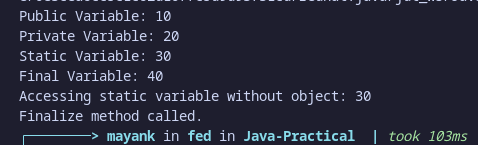
\includegraphics[width=0.8\linewidth]{images/9.png}
    \caption{Example Program Output}
\end{figure}
\setcounter{section}{0}

\practicaltitle{Command Line Arguments}
Command line arguments are parameters passed to the main method when you run a program from the command line.
\section{Syntax}
\subsection{Code: }
\begin{lstlisting}
public static void main(String[] args) {}
\end{lstlisting}
Here, args is an array of String objects that holds the command line arguments passed to the program.

\section{Example of Command Line Argumesnts}
\subsection{Code: }
\begin{lstlisting}
public class CommandLineExample {
    public static void main(String[] args) {
        // Check if any arguments were passed
        if (args.length > 0) {
            System.out.println("Command line arguments:");

            // Iterate over the arguments and print each one
            for (int i = 0; i < args.length; i++) {
                System.out.println
                ("Argument " + i + ": " + args[i]);
            }
        } else {
            System.out.println
            ("No command line arguments were passed.");
        }
    }
}    
\end{lstlisting}
\section{How to Run the Program with Command Line Arguments}
\subsection{Run the program with following command: }
\begin{lstlisting}
java CommandLineExample.java John Jinny Kia
\end{lstlisting}
\subsubsection{Output: }
\begin{figure}[H]
    \centering
    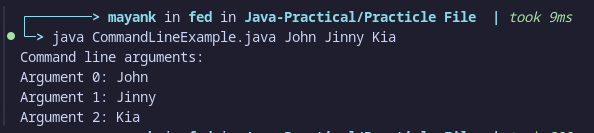
\includegraphics[width=0.9\linewidth]{images/CLA.png}
    \caption{Command Line Arguments}
    \label{fig:sample_image}
\end{figure}

\setcounter{section}{0}

\practicaltitle{Various types of inheritance by applying various access controls to its data members and methods}
Inheritance in Java is a mechanism where a new class (child/subclass) inherits the
properties (fields) and behaviours (methods) of an existing class (parent/superclass). It
promotes code reuse and allows for an organized hierarchy.

\textbf{Types of Inheritance in Java:}
Java supports different types of inheritance, but multiple inheritance (where a class
inherits from more than one class) is not supported directly to avoid ambiguity.
Below are the types Java supports:

\section{Single Inheritance:}
A class inherits from a single superclass.
\subsection{Code: }
\begin{lstlisting}
    class Employee {
        float salary = 40000;
    }

    class Programmer extends Employee {
        int bonus = 10000;
        public static void main(String args[]) {
            Programmer p = new Programmer();
            System.out.println("Programmer salary is:" + p.salary);
            System.out.println("Bonus of Programmer is:" + p.bonus);
        }
    }
\end{lstlisting}

\subsubsection{Output:}
\begin{figure}[H]
    \centering
    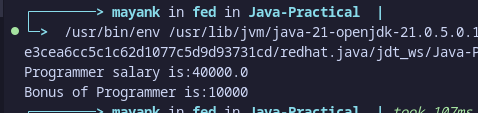
\includegraphics[width=0.9\linewidth]{images/Programmer.png}
    \caption{ouput of Single Inheritance}
    \label{fig:sample_image}
\end{figure}

\section{Multilevel Inheritance:}
A class inherits from a class that is also a subclass of another class, forming a chain of
inheritance.

\subsection{Code: }
\begin{lstlisting}  
class animal {
    public static void eat() {
        System.out.println("Animal eats food");
    }
}

class dog extends animal {
    public static void bark() {
        System.out.println("Dog barks");
    }
}

class puppy extends dog {

    public static void play() {
        System.out.println("Puppy plays");
    }

    public static void main(String[] args) {
        puppy obj = new puppy();
        obj.eat();
        obj.bark();
        obj.play();
    }
}
\end{lstlisting}

\subsubsection{Output:}
\begin{figure}[H]
    \centering
    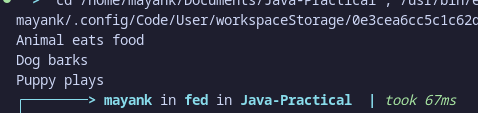
\includegraphics[width=0.9\linewidth]{images/puppy.png}
    \caption{ouput of Multilevel Inheritance}
    \label{fig:sample_image}
\end{figure}

\section{Hierarchical Inheritance:}
Multiple classes inherit from a single superclass.

\subsection{Code: }
\begin{lstlisting}  
class Animal {
    public void eat() {
        System.out.println("Animal eats");
    }
}

class Dog extends Animal {
    public void bark() {
        System.out.println("Dog barks");
    }
}

class Cat extends Animal {
    public void meow() {
        System.out.println("Cat meows");
    }
}

public class HInherit {
    public static void main(String[] args) {
        // Create Dog object and callmethods
        Dog dog = new Dog();
        dog.eat(); // Inherited method from Animal
        dog.bark(); // Specific method of Dog
        // Create Cat object and call methods 
        Cat cat = new Cat();
        cat.eat(); // Inherited method from Animal
        cat.meow(); // Specific method of Cat
    }
}
\end{lstlisting}

\subsubsection{Output:}
\begin{figure}[H]
    \centering
    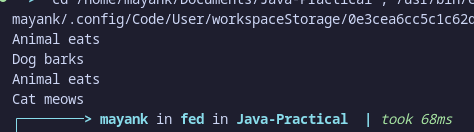
\includegraphics[width=0.9\linewidth]{images/HInherit.png}
    \caption{ouput of Hierarchical Inheritance}
    \label{fig:sample_image}
\end{figure}

\setcounter{section}{0}

\practicaltitle{Method overriding}
Method overriding in Java is a key concept of Object-Oriented Programming (OOP), where a subclass (child class) provides a specific implementation of a method that is already defined in its superclass (parent class). The method in the subclass should have the same name, return type, and parameters as in the superclass. The idea is to allow a subclass to modify or enhance the behavior of the method that it inherits from its parent class

\section{Example Using Code: }
\begin{lstlisting}
    class Car {
        public String bestModel() {
            return "";
        }
    }
    
    class BMW extends Car {
        @Override
        public String bestModel() {
            return "M4 Competition";
        }
    }
    
    class Audi extends Car {
        @Override
        public String bestModel() {
            return "RS7";
        }
    }
    
    class Porsche extends Car {
        @Override
        public String bestModel() {
            return "911 gt3rs";
        }
    }
    
    public class MetOvr {
        public static void main(String[] args) {
            BMW bmw = new BMW();
            Audi audi = new Audi();
            Porsche porsche = new Porsche();
    
            System.out.println(bmw.bestModel());
            System.out.println(audi.bestModel());
            System.out.println(porsche.bestModel());
        }
    }    
\end{lstlisting}
\subsubsection{Output: }
\begin{figure}[H]
    \centering
    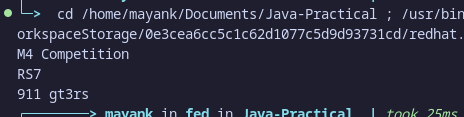
\includegraphics[width=0.9\linewidth]{images/MetOvrr.png}
    \caption{ouput of Method overriding}
    \label{fig:sample_image}
\end{figure}

\subsubsection{Example of Method overriding by Diagram: }
\begin{figure}[H]
    \centering
    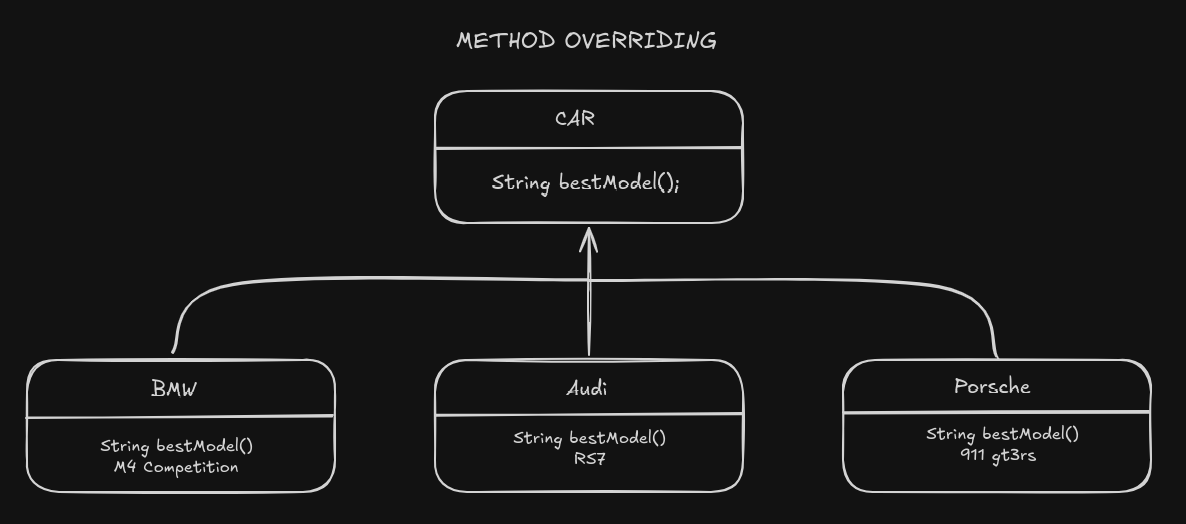
\includegraphics[width=0.9\linewidth]{images/mETHODdIAGRAM.png}
    \caption{Example of Method overriding}
    \label{fig:sample_image}
\end{figure}

\setcounter{section}{0}

\practicaltitle{Abstract class}
An abstract class in Java is a class that cannot be instantiated on its own. It is used to represent an abstract concept that other classes can inherit from, providing a common structure. An abstract class can have both abstract methods (methods without a body, meant to be implemented by subclasses) and concrete methods (methods with a body)

\section{Syntax: }
\begin{lstlisting}
    abstract class ClassName {
    // Abstract method (no body)
    public abstract void methodName();

    // Concrete method (with body)
    public void anotherMethod() {
        System.out.println("This is a concrete method.");
    }
}
\end{lstlisting}

\subsection{Code: }
\begin{lstlisting}
abstract class Payment {
    public abstract void makePayment(double amount);

    public void paymentDetails(double amount) {
        System.out.println("Payment of $" + amount + " is being processed.");
    }
}

class CreditCardPayment extends Payment {
    @Override
    public void makePayment(double amount) {
        System.out.println("Processing Credit Card Payment of $" + amount);
    }
}

class PayPalPayment extends Payment {
    @Override
    public void makePayment(double amount) {
        System.out.println("Processing PayPal Payment of $" + amount);
    }
}

public class Abs {
    public static void main(String[] args) {
        Payment creditCard = new CreditCardPayment();
        Payment payPal = new PayPalPayment();
    
        creditCard.paymentDetails(100.50);
        creditCard.makePayment(100.50);   
    
        System.out.println(); 
    
        payPal.paymentDetails(50.75);  
        payPal.makePayment(50.75);     
    }
}
\end{lstlisting}
\subsubsection{Output: }
\begin{figure}[H]
    \centering
    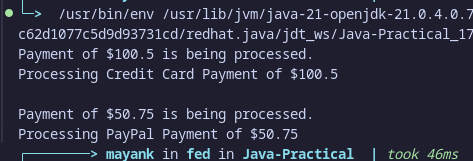
\includegraphics[width=0.9\linewidth]{images/AbsOut.png}
    \caption{ouput of abstract class}
    \label{fig:sample_image}
\end{figure}

\setcounter{section}{0}

\practicaltitle{Nested class}
A nested class in Java is a class defined within another class. Nested classes can be
used to logically group classes that are only used in one place, improving
encapsulation and making the code more readable. Nested classes have access to the
members (both static and non- static) of the outer class, depending on whether they are
static or non-static themselves.

\section{Static Nested Class :}
A static nested class in Java is a nested class that is declared static. Since it is a static
member of the outer class, it can be accessed without creating an instance of the outer
class.
However, unlike non-static inner classes, a static nested class cannot access non-static
members (fields or methods) of the outer class directly. It can only access the static
members (both fields and methods) of the outer class.

\subsection{Code: }
\begin{lstlisting}
class outerClass {
    static int outer_x = 34; // Static member
    int outer_y = 102;
    // Non-static member
    private static int outerPrivate = 44; // Static member
    static class innerClass {
        // Static nested class
        void display() {
            outerClass outer = new outerClass();
            System.out.println("Value of x: " + outer_x);
            System.out.println("Value of y: " + outer.outer_y);
            System.out.println("Value of private variable: " + outerPrivate);
        }
    }
}

public class Nest { // Separate class to run the main method
    public static void main(String[] args) {
        System.out.println("Static Nested Class");
        outerClass.innerClass obj = new outerClass.innerClass();
        obj.display(); // Call the display method}
    }
}
\end{lstlisting}
\subsubsection{Output: }
\begin{figure}[H]
    \centering
    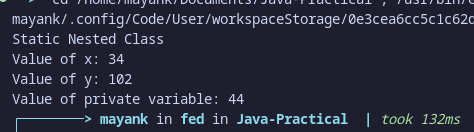
\includegraphics[width=0.9\linewidth]{images/nest.png}
    \caption{ouput of nested class}
    \label{fig:sample_image}
\end{figure}

\setcounter{section}{0}

\practicaltitle{Constructor chaining}
In Java, constructor chaining is a sequence of invoking constructors upon initializing an object. It is used when we want to invoke a number of constructors, one after another by using only an instance.

% \section{Static Nested Class :}
\subsection{Code: }
\begin{lstlisting}
class Animal {
    String name;
    String speak;

    Animal(){
        this("Cat", "Meow");
        System.out.println("This is Default Constructor");
    }

    Animal(String name, String speak) {
        this.name = name;
        this.speak = speak;
        System.out.println("This is Parameterised Constructor");
        System.out.println(name + " | " + speak);
    }
}

public class Chain {
    public static void main(String[] args) {
        Animal obj1 = new Animal();
    }
}
\end{lstlisting}
\subsubsection{Output: }
\begin{figure}[H]
    \centering
    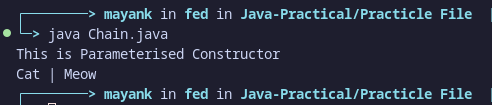
\includegraphics[width=0.9\linewidth]{images/Chain.png}
    \caption{ouput of constructor chaining}
    \label{fig:sample_image}
\end{figure}

\setcounter{section}{0}
\practicaltitle{Importing Classes from User-defined Package and Creating Packages Using Access Protection}

\section{Packages}
In Java, a package is a namespace that organizes a set of related classes and interfaces. Packages serve as containers for classes, helping to avoid name conflicts and making code easier to locate and manage. Java’s standard library is organized into packages (like \texttt{java.util} or \texttt{java.io}), allowing developers to reuse classes easily without having to rewrite common functionalities. By using packages, we can logically separate different components of a program and control their visibility to other classes.

Packages also play a critical role in implementing access control. Java provides four levels of access control: \textbf{public}, \textbf{protected}, \textbf{default} (package-private), and \textbf{private}. These access levels determine how classes and members (fields and methods) can be accessed across different packages.

\begin{itemize}
    \item \textbf{Public}: Accessible from any other class, irrespective of the package.
    \item \textbf{Protected}: Accessible within the same package and by subclasses in other packages.
    \item \textbf{Default (Package-private)}: Accessible only within the same package; no modifier is needed.
    \item \textbf{Private}: Accessible only within the class in which it is defined.
\end{itemize}

\section{Creating and Importing a User-defined Package}

The following code demonstrates how to define a package, create a class within the package with various access levels, and then import and use that class in a main program.

\subsection{Code for the Package (\texttt{mypackage/MyClass.java}):}

\begin{lstlisting}[language=Java]
package mypackage;

public class MyClass {
    public int publicVar = 10;
    protected int protectedVar = 20;
    int defaultVar = 30; // default access
    private int privateVar = 40;

    public void display() {
        System.out.println("Public variable: " + publicVar);
        System.out.println("Protected variable: " + protectedVar);
        System.out.println("Default variable: " + defaultVar);
        System.out.println("Private variable: " + privateVar);
    }
}
\end{lstlisting}

\subsection{Code for Importing the Package (\texttt{ImportPackage.java}):}

\begin{lstlisting}[language=Java]
import mypackage.MyClass;

public class ImportPackage {
    public static void main(String[] args) {
        MyClass obj = new MyClass();
        
        // Accessing variables with different access modifiers
        System.out.println("Accessing public variable: " + obj.publicVar);
        // System.out.println("Accessing protected variable: " + obj.protectedVar); // Error: Not accessible
        // System.out.println("Accessing default variable: " + obj.defaultVar); // Error: Not accessible
        // System.out.println("Accessing private variable: " + obj.privateVar); // Error: Not accessible

        obj.display(); // Method displays all variables within the same class
    }
}
\end{lstlisting}

\subsection{Output:}
\begin{figure}[H]
    \centering
    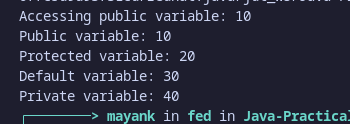
\includegraphics[width=0.8\linewidth]{images/29.png}
    \caption{Output demonstrating access control when importing from a user-defined package}
\end{figure}


\setcounter{section}{0}

\practicaltitle{Interfaces, nested interfaces and use of extending interfaces}
In Java, an interface is a reference type that is similar to a class but is used to specify a
set of abstract methods (methods without a body). Interfaces define what a class must
do but not how it does it. Any class that implements an interface must provide an
implementation for all of its abstract methods.
\subsection{Code: }
\begin{lstlisting}
    interface Printable {
        // Defining an interface 
        void print(); // Abstract method
    }
    
    class Document implements Printable {
    
        @Override
        public void print() {
            System.out.println("Printing a document ...");
        }
    }
    
    class Image implements Printable {
    
        @Override
        public void print() {
            System.out.println("Printing an image...");
        }
    }
    
    public class InterfaceExample {
    
        public static void main(String[] args) {
            // Creating objects of classes that implement the Printable interface
            Printable doc = new Document();
            Printable img = new Image();
            // Calling the print method using interface references
            doc.print();
            img.print();
        }
    }
\end{lstlisting}
\subsubsection{Output: }
\begin{figure}[H]
    \centering
    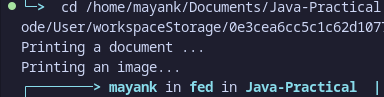
\includegraphics[width=0.9\linewidth]{images/Interface.png}
    \caption{ouput of interface}
    \label{fig:sample_image}
\end{figure}

\section{Nested Interfaces}
A nested interface in Java is an interface that is declared within another interface or
class. This allows better organization of code, especially when the interface is only
relevant in the context of the enclosing class or interface.


\begin{lstlisting}

    class Vehicle { // Outer class

    interface Engine { // Nested

        void start();

        void stop();
    }

    // Method to demonstrate the nested interface
    public void useEngine() {
        // Implementing the nested interface
        Engine engine = new Engine() {
            @Override
            public void start() {
                System.out.println("Engine is starting...");
            }

            @Override
            public void stop() {
                System.out.println("Engine is stopping...");
            }

        };
        engine.start();
        engine.stop();
    }
}

public class Main {

    public static void main(String[] args) {
        System.out.println("Nested Interface (Interface within Class)");
        Vehicle vehicle = new Vehicle();
        // Using the nested interface
        vehicle.useEngine();
    }
}

\end{lstlisting}
\begin{figure}[H]
    \centering
    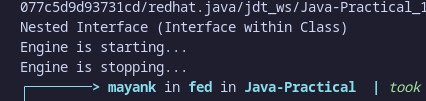
\includegraphics[width=0.9\linewidth]{images/NestedInter.png}
    \caption{ouput of nested interface}
    \label{fig:sample_image}
\end{figure}

\section{Extended Interfaces}


\begin{lstlisting}    
interface Animal { // Outer interface 
void sound();
interface Behavior { // Nested interface 
    void eat();
}
}

class Dog implements Animal, Animal.Behavior {

@Override
public void sound() {
    System.out.println("Dog barks");
}

// Implementing the eat method from the nested interface
@Override
public void eat() {
    System.out.println("Dog eats dog food");
}
}

public class Inter {

public static void main(String[] args) {
    System.out.println("Nested Interface(Interface within Interface )");
    Dog dog = new Dog();
    dog.sound(); // Call the soundmethod dog
    dog.eat(); // Call the eat

}
}

\end{lstlisting}
\begin{figure}[H]
    \centering
    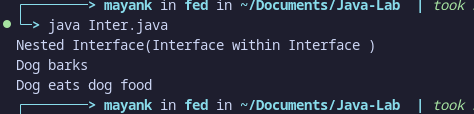
\includegraphics[width=0.9\linewidth]{images/Inter.png}
    \caption{ouput of Extended interface}
    \label{fig:sample_image}
\end{figure}

\setcounter{section}{0}
\practicaltitle{Exception Handling - Using Predefined Exception}

\section{Exceptions}
In Java, Exception is an unwanted or unexpected event, which occurs during the execution of a program, i.e. at run time, that disrupts the normal flow of the program’s instructions. Exceptions can be caught and handled by the program. When an exception occurs within a method, it creates an object. This object is called the exception object. It contains information about the exception, such as the name and description of the exception and the state of the program when the exception occurred.


Major reasons why an exception Occurs:
\begin{itemize}
    \item Invalid user input
    \item Device failure
    \item Loss of network connection
    \item Physical limitations (out-of-disk memory)
    \item Code errors
    \item Out of bound
    \item Null reference
    \item Type mismatch
    \item Opening an unavailable file
    \item Database errors
    \item Arithmetic errors
\end{itemize}

\section{Errors}
Errors represent irrecoverable conditions such as Java virtual machine (JVM) running out of memory, memory leaks, stack overflow errors, library incompatibility, infinite recursion, etc. Errors are usually beyond the control of the programmer, and we should not try to handle errors.

\section{Exception Handling}
Exception handling in Java is a mechanism used to handle runtime errors, allowing the normal flow of the application to be maintained. Java provides a set of predefined exceptions in the \texttt{java.lang} package, which can handle common runtime errors, such as \texttt{ArithmeticException}, \texttt{NullPointerException} and more. These exceptions are part of Java's standard library and extend the \texttt{Exception} class.


\section{Example Code for Exception Handling Using Predefined Exception}

The following code demonstrates handling an \texttt{ArithmeticException} using a \texttt{try-catch} block.

\subsection{Code:}

\begin{lstlisting}[language=Java]
public class ExceptionHandling {
    public static void main(String[] args) {
        int a = 10;
        int b = 0;

        try {
            int result = a / b; // This will cause an ArithmeticException
            System.out.println("Result: " + result);
        } catch (ArithmeticException e) {
            System.out.println("Exception caught: Division by zero is not allowed.");
            System.out.println("Error: " + e);
        }

        System.out.println("Program continues after handling the exception.");
    }
}
\end{lstlisting}

\subsection{Output:}
\begin{figure}[H]
    \centering
    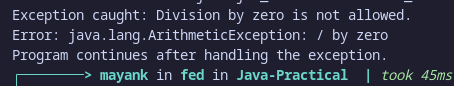
\includegraphics[width=0.8\linewidth]{images/30.png}
    \caption{Output demonstrating exception handling for ArithmeticException in Java}
\end{figure}

\setcounter{section}{0}
\practicaltitle{Exception Handling - Creating User-defined Exceptions}

\section{User Defined Exceptions}
In Java, we can create custom exceptions (user-defined exceptions) by extending the \texttt{Exception} class. User-defined exceptions allow developers to create exceptions specific to the application's needs, providing more meaningful error messages and handling unique error conditions.

A user-defined exception is created by defining a new class that extends \texttt{Exception} or any of its subclasses. By overriding the \texttt{Exception} class’s constructors, we can customize the exception message and implement specific behaviors for our custom exception.

\section{Throw Keyword}
Java’s exception-handling mechanism includes the throw keyword, which is used to explicitly throw an exception. Exceptions can be thrown in two ways:
\begin{itemize}
    \item \textbf{Implicit Throwing}: This occurs when the Java runtime system automatically throws an exception in response to common errors (e.g., \texttt{NullPointerException} or \texttt{ArithmeticException}).
    \item \textbf{Explicit Throwing}: Using the throw keyword, developers can explicitly throw an exception when a specific condition is met. This is often used with user-defined exceptions to control error handling based on custom logic.
\end{itemize}

For example, we can create an exception that will be thrown if a user enters an invalid input, such as an age below a certain threshold. The throw keyword enables us to control precisely when and where an exception occurs, ensuring more robust error handling.



\section{Example Code for User-defined Exception}

The following code demonstrates how to define and use a custom exception in Java.

\subsection{Code:}

\begin{lstlisting}[language=Java]
public class UserDefinedException {
    public static void main(String[] args) {
        try {
            checkAge(15); // This will throw an InvalidAgeException
        } catch (InvalidAgeException e) {
            System.out.println("Exception caught: " + e.getMessage());
        }

        System.out.println("Program continues after handling the exception.");
    }

    // Method to check age
    static void checkAge(int age) throws InvalidAgeException {
        if (age < 18) {
            throw new InvalidAgeException("Age must be 18 or above.");
        }
        System.out.println("Age is valid.");
    }
}

// Custom exception class
class InvalidAgeException extends Exception {
    public InvalidAgeException(String message) {
        super(message);
    }
}
\end{lstlisting}

\subsection{Output:}
\begin{figure}[H]
    \centering
    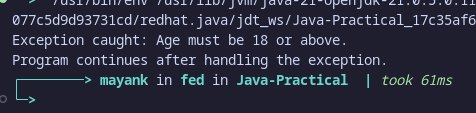
\includegraphics[width=0.8\linewidth]{images/31.png}
    \caption{Output demonstrating a user-defined exception in Java}
\end{figure}

\setcounter{section}{0}
\practicaltitle{Multithreading by extending Thread Class}

\section{Program: }
\begin{lstlisting}
    class EvenThread extends Thread{
        @Override
        public void run() {
            for (int i = 0; i < 10; i++) {
                    System.err.println("Even Thread");
                    try {
                        Thread.sleep(10);
                    } catch (InterruptedException e) {
                        e.printStackTrace();
                    }
            }
        }
    }
    
    class OddThread extends Thread{
        @Override
        public void run() {
            for (int i = 0; i < 10; i++) {
                    System.err.println("Odd Thread");
                    try {
                        Thread.sleep(10);
                    } catch (InterruptedException e) {
                        e.printStackTrace();
                    }
                
            }
        }
    }
    public class MultiThread {
        public static void main(String[] args) {
            Thread odd = new OddThread();
            Thread even = new EvenThread();
    
            even.start();
            odd.start();
        }
        
    }
\end{lstlisting}

\subsection{Ouptut: }
\begin{figure}[H]
    \centering
    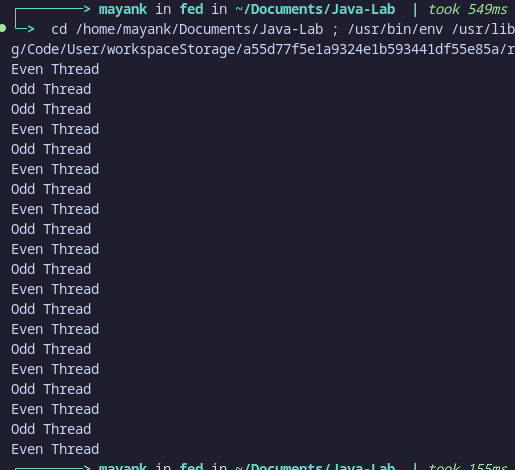
\includegraphics[width=0.8\linewidth]{images/Thread.png}
    \caption{Multithreading using thread class}
\end{figure}


\setcounter{section}{0}
\practicaltitle{Multithreading by implementing Runnable Interface}

\section{Program: }
\begin{lstlisting}

    public class LambdaThread {

    public static void main(String[] args) {
        Runnable obj1 = () -> {
            for (int i = 0; i < 6; i++) {
                System.err.println("Thread 1");
                try {
                    Thread.sleep(10);
                } catch (InterruptedException e) {
                    e.printStackTrace();
                }
            }
        };
        Runnable obj2 = () -> {
            for (int i = 0; i < 6; i++) {
                System.err.println("Thread 2");
                try {
                    Thread.sleep(10);
                } catch (InterruptedException e) {
                    e.printStackTrace();
                }
            }
        };

        Thread t1 = new Thread(obj1);
        Thread t2 = new Thread(obj2);

        t1.start();
        t2.start();
    }
}

\end{lstlisting}

\subsection{Ouptut: }
\begin{figure}[H]
    \centering
    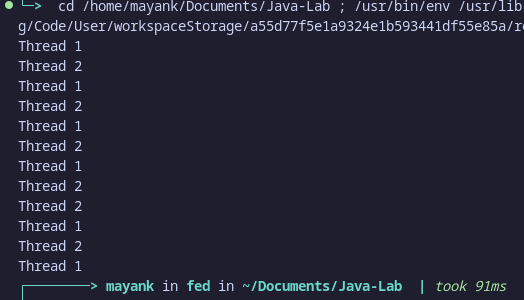
\includegraphics[width=0.8\linewidth]{images/Runnable.png}
    \caption{Mutli threading using runnable interface}
\end{figure}

\setcounter{section}{0}
\practicaltitle{Thread life cycle}
\section{Thread States}
\begin{itemize}
    \item New State
    \item Runnable State
    \item Blocked State
    \item Waiting State
    \item Terminated State
\end{itemize}

\begin{lstlisting}
    // Java program to demonstrate thread states
class thread implements Runnable {
    public void run()
    {
        // moving thread2 to timed waiting state
        try {
            Thread.sleep(1500);
        }
        catch (InterruptedException e) {
            e.printStackTrace();
        }

        System.out.println(
            "State of thread1 while it called join() method on thread2 -"
            + Test.thread1.getState());
        try {
            Thread.sleep(200);
        }
        catch (InterruptedException e) {
            e.printStackTrace();
        }
    }
}

public class Test implements Runnable {
    public static Thread thread1;
    public static Test obj;

    public static void main(String[] args)
    {
        obj = new Test();
        thread1 = new Thread(obj);

        // thread1 created and is currently in the NEW
        // state.
        System.out.println(
            "State of thread1 after creating it - "
            + thread1.getState());
        thread1.start();

        // thread1 moved to Runnable state
        System.out.println(
            "State of thread1 after calling .start() method on it - "
            + thread1.getState());
    }

    public void run()
    {
        thread myThread = new thread();
        Thread thread2 = new Thread(myThread);

        // thread2 created and is currently in the NEW
        // state.
        System.out.println(
            "State of thread2 after creating it - "
            + thread2.getState());
        thread2.start();

        // thread2 moved to Runnable state
        System.out.println(
            "State of thread2 after calling .start() method on it - "
            + thread2.getState());

        // moving thread2 to timed waiting state
        try {
            // moving thread2 to timed waiting state
            Thread.sleep(200);
        }
        catch (InterruptedException e) {
            e.printStackTrace();
        }
        System.out.println(
            "State of thread2 after calling .sleep() method on it - "
            + thread2.getState());

        try {
            // waiting for thread2 to die
            thread2.join();
        }
        catch (InterruptedException e) {
            e.printStackTrace();
        }
        System.out.println(
            "State of thread2 when it has finished it's execution - "
            + thread2.getState());
    }
}
\end{lstlisting}
\subsection{Ouptut: }
\begin{figure}[H]
    \centering
    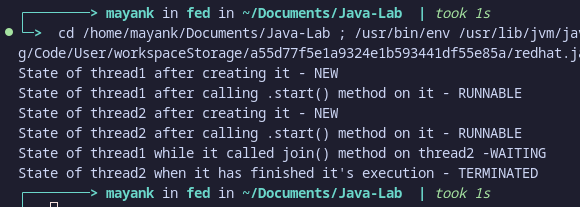
\includegraphics[width=0.8\linewidth]{images/Life.png}
    \caption{Thread Life Cycle}
\end{figure}

\setcounter{section}{0}
\practicaltitle{StringBuffer class and its methods}
StringBuffer is a class in Java that represents a mutable sequence of characters. It provides an alternative to the immutable String class, allowing you to modify the contents of a string without creating a new object every time.

\section{Append Method}

\subsection{Code:}
\begin{lstlisting}
    public class StringBufferAppend {
        public static void main(String[] args)
        {
            // Append Method
            StringBuffer sb = new StringBuffer();
            sb.append("Hello");
            sb.append(" ");
            sb.append("world");
            String message = sb.toString();
            System.out.println(message);
        }
    }    
\end{lstlisting}

\subsubsection{Output:}
\begin{figure}[H]
    \centering
    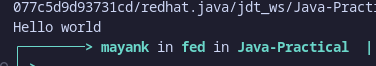
\includegraphics[width=0.8\linewidth]{images/41.png}
    \caption{Append Method}
\end{figure}

\section{Insert Method}
\subsection{Code:}
\begin{lstlisting}
public class StringBufferInsert {
    // Insert Method in String Buffer
    public static void main(String[] args) {
        StringBuffer sb = new StringBuffer("Hello");
        sb.insert(3, "HHH");
        String message = sb.toString();
        System.out.println(message);
    }
}
\end{lstlisting}

\subsubsection{Output:}
\begin{figure}[H]
    \centering
    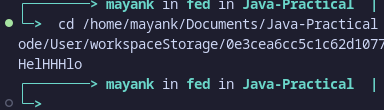
\includegraphics[width=0.8\linewidth]{images/42.png}
    \caption{Insert Method}
\end{figure}

\section{Replace Method}
\subsection{Code:}
\begin{lstlisting}
public class StringBufferReplace {
    // Replace Method in String Buffer
    public static void main(String[] args) {
        StringBuffer sb = new StringBuffer("Hello World");
        sb.replace(6, 11, "Java");
        String message = sb.toString();
        System.out.println(message);
    }
}
\end{lstlisting}
\subsubsection{Output:}
\begin{figure}[H]
    \centering
    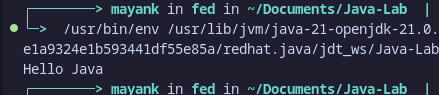
\includegraphics[width=0.8\linewidth]{images/replace.png}
    \caption{Delete Method}
\end{figure}

\section{Delete Method}
\subsection{Code:}
\begin{lstlisting}
public class StringBufferDelete {
    // Delete Method in String Buffer
    public static void main(String[] args) {
        StringBuffer sb = new StringBuffer("Hello World");
        sb.delete(5, 11);
        String message = sb.toString();
        System.out.println(message);
    }
}
\end{lstlisting}
\subsubsection{Output:}
\begin{figure}[H]
    \centering
    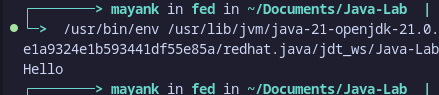
\includegraphics[width=0.8\linewidth]{images/DElete.png}
    \caption{Delete Method}
\end{figure}

\section{Reverse Method}
\subsection{Code:}
\begin{lstlisting}
public class StringBufferReverse {
    // Reverse Method in String Buffer
    public static void main(String[] args) {
        StringBuffer sb = new StringBuffer("Hello");
        sb.reverse();
        String message = sb.toString();
        System.out.println(message);
    }
}
\end{lstlisting}
\subsubsection{Output:}
\begin{figure}[H]
    \centering
    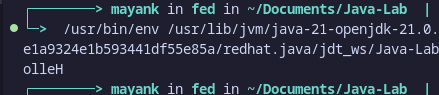
\includegraphics[width=0.8\linewidth]{images/reverse.png}
    \caption{Reverse Method}
\end{figure}

\end{document}